\documentclass[]{article}
\usepackage[utf8]{inputenc}
\usepackage{graphicx}
\usepackage{amsmath}
\usepackage{amsfonts}
\usepackage{amssymb}
\usepackage{subcaption}
%opening
\title{Homework 2}
\author{Ian Hunt-Isaak}
\date{}
\begin{document}

\maketitle


\section{Introduction}
The continuity equation:
\begin{equation}
\frac{\partial}{\partial t} \varphi + \nabla(\varphi \vec{u}) = 0,
\label{eq:continuity}
\end{equation}
with $\varphi$ the value of interest and $\vec{u}$ the velocity field,  is a special case of a conservation equation, in which there are no diffusion or source terms. are those that describe the transport of some physical quantity. This equation describes the flow of an incompressible fluid, such as water, and therefore is a highly useful equation to be able to solve numerically. Unfortunately even something as simple as the continuity equation, Eq. \ref{eq:continuity}, can be incredibly difficult to approach numerically. In simulating this we have the familiar constraint of stability, i.e. that the solution values will not explode, and we also require that our values be positive for all time and space. This latter requirement comes from the fact that when simulating mass transport it would be physically meaningless to have negative matter. 
Without a diffusive term 




\section{Numerical Methods}
In 1-D there are ways to discretize the derivatives in Eq. \ref{eq:continuity}, with the most obvious being the centered difference or upwind approaches. Unfortunately in the case of the purely advective system we are considering the centered difference method will lead to an unstable solution. This could be considered to arise from the fact that in order to do this 

The stability of the solution for the upwind time marching scheme will be determined by the CFL number with $\frac{u \Delta t}{\Delta X}\leq 1$
\section{Understanding SHASTA}
As presented by Boris and Book \cite{shasta} the SHASTA algorithm is very similar to the Flux Corrected Transport with explicit $\frac{1}{8}$ antidiffusion. However, instead of simply subtracting an antidiffusive quantity of equal magnitude to the diffusion introduced by the FCT scheme Boris and Book design a correction that prevents the creation of new local extrema. After the first step of FCT the correction is:
\begin{equation}
\bar{\varphi}^n_j = \varphi_j^n + f^c_{j-\frac{1}{2}}-f^c_{j+\frac{1}{2}},
\end{equation}
where $\bar{\varphi}^n_j$ is the corrected value and the $f^c$ are defined below so as to prevent the creation of local extrema. With $\Delta_{j+\frac{1}{2}} = \varphi^n_{j+1} - \varphi^n_{j}$, $\Delta_{j-\frac{1}{2}} = \varphi^n_{j} - \varphi^n_{j-1}$, and $\Delta_{j\pm\frac{3}{2}}$ defined similarly we can define $f^c$ as follows:

\begin{equation}
f^c_{j+\frac{1}{2}} = sgn(\Delta_{j+\frac{1}{2}}) \text{Max}\left(0,\text{Min}\left(\Delta_{j-\frac{1}{2}} sgn(\Delta_{j+\frac{1}{2}}), \frac{1}{8}|\Delta_{j+\frac{1}{2}}|,\Delta_{j+\frac{3}{2}} sgn(\Delta_{j+\frac{1}{2}}\right)\right)
\label{eq:def_fc_right}
\end{equation}
This equation considers where "mass" could have gone from, or come into point $j$ due to numerical diffusion. It then selects the smallest possible correction with a sign chosen based on the relative magnitudes of $\varphi^n_{j+1}$ and $\varphi^n_{j}$. While, Boris and Book do not provide an equation for $f^c_{j-\frac{1}{2}}$ by considering the intention of how the correction term works we can construct it as follows:

\begin{equation}
f^c_{j-\frac{1}{2}} = sgn(\Delta_{j-\frac{1}{2}}) \text{Max}\left(0,\text{Min}\left(\Delta_{j+\frac{1}{2}} sgn(\Delta_{j-\frac{1}{2}}), \frac{1}{8}|\Delta_{j-\frac{1}{2}}|,\Delta_{j-\frac{3}{2}} sgn(\Delta_{j-\frac{1}{2}}\right)\right).
\label{eq:def_fc_left}
\end{equation}
This construction of $f^c_{j-\frac{1}{2}}$ is the only one that maintains the symmetry of the corrective equation, simply shifting the subscript values by -1 would not be result in proper correction to the FCT method. 

\section{Results}
A square waveform being advected to the right was simulated using the upwind, Lax-Wendroff, Flux Corrected Transport(FCT), FCT + Antidiffusion, and the FCT + Boris and Book correction methods. A comparison of the results of each of these methods can be seen in Figures \ref{fig:constU_f_compare}, and \ref{fig:constU_f_compare_offset}. As expected the upwind scheme does not induce wiggles in the solution, however it does suffer from a numerical diffusion causing the initial square waveform to degrade into a Gaussian waveform. 


\begin{figure}
		\centering
		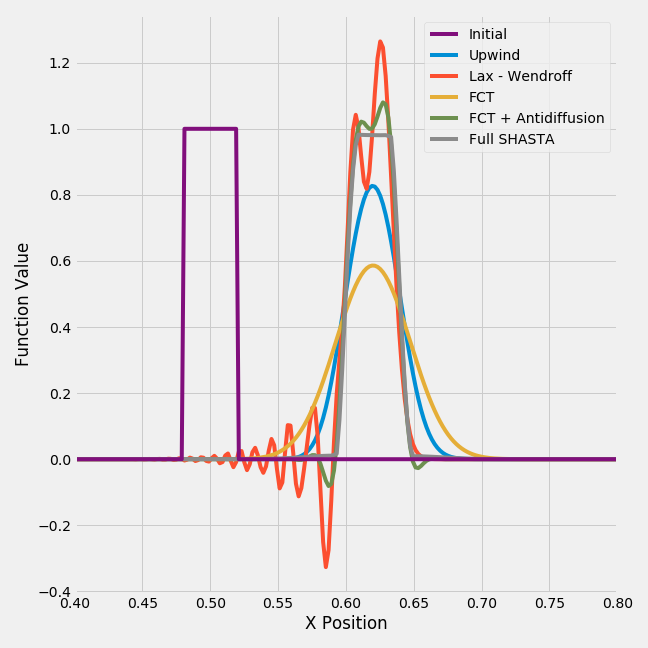
\includegraphics[width=.8\linewidth]{figures/constU_fCompare.png}

	\caption{Comparison of the different approaches to numerically solving Eq. \ref{eq:continuity}. In this comparison we can see that the center of mass is propagated at the same velocity regardless of the time marching method or corrective diffusion steps used. For an easier comparison of profile shapes consider Figure \ref{fig:constU_f_compare_offset}. }
	\label{fig:constU_f_compare}
\end{figure}
\begin{figure}
	\centering
	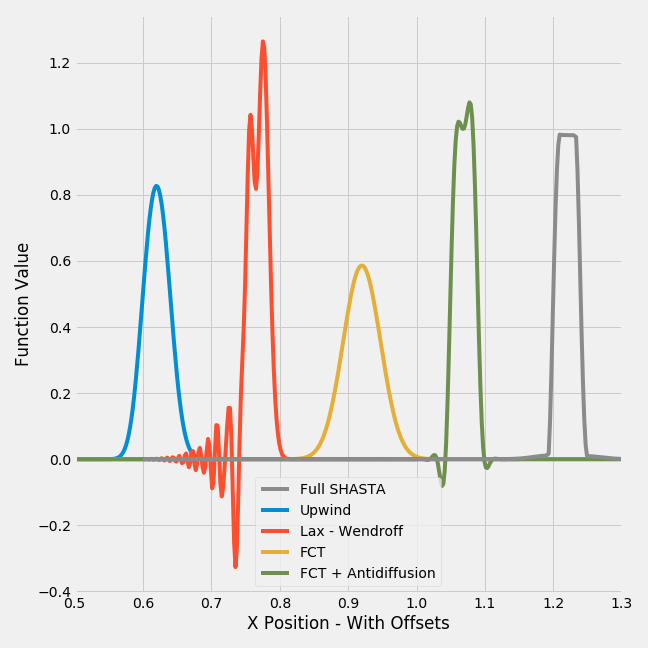
\includegraphics[width=.8\linewidth]{figures/constU_fCompare_offset.png}
	\caption{Comparison of the different approaches to numerically solving Eq. \ref{eq:continuity} after 600 time steps with an initial wave form of a square wave. In this comparison the waveforms have been offset in X from each other so as to compare their shape. Overall the results of this comparison are as expected, with both the Upwind and FCT methods showing strong dispersion, Lax-Wendroff ad FCT + Antidiffusion maintaining the basic square wave shape, but with wiggles, and finally the SHASTA method developed by Boris and Book providing the most accurate results. A comparison of the level diffusion in each method can be seen in Figure \ref{fig:constU_compareH}. }
	\label{fig:constU_f_compare_offset}
\end{figure}
\begin{figure}

		\centering
		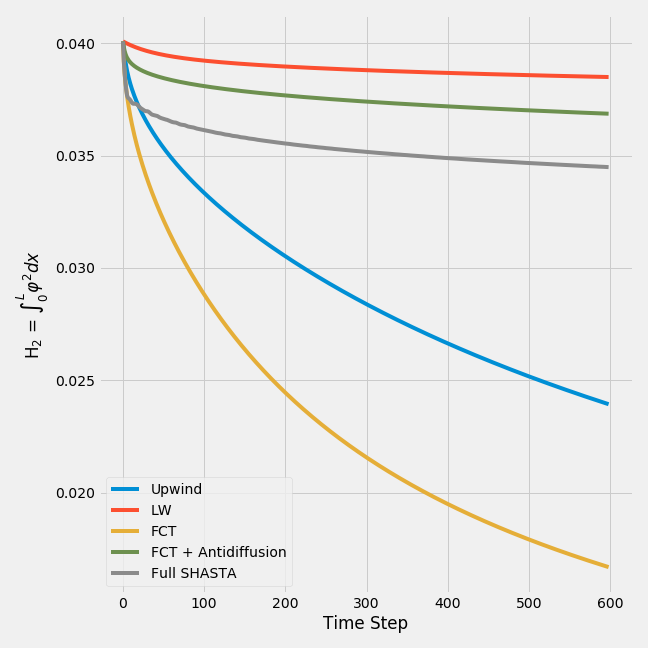
\includegraphics[width=.8\linewidth]{figures/constU_compareH.png}
		\caption{Comparison of the quantity $H_2$, which serves as a measure of the localization (or entropy) of the solution. In this case we can use this as a proxy measure for the amount of numerical diffusion introduced by our solution method, with lower values of $H_2$ corresponding to greater amounts of diffusion. The results here agree with visual inspection of Figure \ref{fig:constU_f_compare_offset}, though they provide a more quantitative sense of the differences of diffusion in the methods. While the SHASTA method is unquestionably the most accurate we can see here that while avoiding wiggles, it does less well than Lax-Wendroff or FCT+Antidiffusion at preventing numerical diffusion.}
	\label{fig:constU_compareH}
\end{figure}

  \begin{thebibliography}{1}
  	
  	\bibitem{shasta} Boris, J. P. \& Book, D. L. Flux-corrected transport. I. SHASTA, a fluid transport algorithm that works. Journal of computational physics 11, 38–69 (1973).
  	

  \end{thebibliography}



\end{document}
